\section{Background Information}
\subsection{Histograms of Oriented Gradients}\label{sec:hog}

The HOG descriptor is excellent at pedestrian detection because it prioritizes the most discriminative qualities of any pedestrian - their shape: limbs, head, and other features with prominent edges \cite{dalal_2005_histograms}, unlike other feature descriptors like HaaR wavelets which are colloquially described as “texture features” \cite{zia_2015_why}.

\subsubsection{One Fundamental Property of Images}

At their core, images are matrices of color channel intensity values \cite{rein_image_definition} and thus an edge can be understood as a region in which there is a change of intensity. In figure \ref{fig:pixel_intensity} an edge is characterized by the steepness of the pixel intensity function's gradient, as gradient values are greater at the edges/corners of an object rather than homogeneous areas \cite{niebles2012edge}. As such, gradients may highlight the contours of objects and discard noise/texture information, precisely what is needed in pedestrian detection.

\begin{figure}
    \centering
    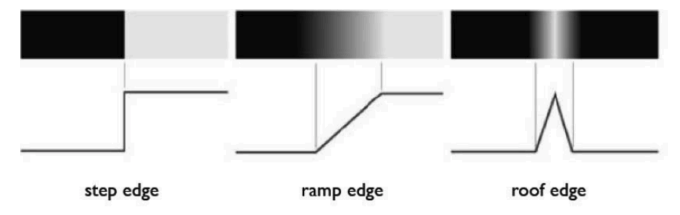
\includegraphics[width=0.75\linewidth]{images/pixel_intensity.png}
    \caption{Representation of the three types of edge that can be found in image analysis. Each intensity function is mapped to a row's pixel intensity values. Source: \cite{niebles2012edge}}
    \label{fig:pixel_intensity}
\end{figure}

\subsubsection{Gradient Computation}\label{sec:deriv_mask}

In HOG, a derivative mask \footnote{The term "derivative mask" appears to be only used in the seminal HOG paper \cite{dalal_2005_histograms}. In most computer vision literature, it is said that convolution is performed with a filter or kernel \cite{niebles2012edge}.}  is used to compute gradient information from an image \cite{dalal_2005_histograms} by performing convolution, the process of adding each element of the image to its local neighbors, weighted by the mask \cite{niebles2012edge}, as shown in equation \ref{eq:convolution}, where $I$ is the image matrix, $K$ the mask's matrix and $k$ - the "radius" of $K$ \footnote{In convolution, the "radius" of a mask is defined as the distance from the center element to an edge element. \cite{niebles2012edge}}.

\begin{equation}\label{eq:convolution}
    F(x,y) = \sum_{i=-k}^{k} \sum_{j=-k}^{k} I(x+i,y+j) \cdot K(i,j)
\end{equation}

It was shown that a simple 1D derivative mask of form $[-1,0,1]$, formally called a central discrete derivative \cite{niebles2012edge}, while requiring less computation than $3\times3$ Sobel or $2\times2$ diagonal masks, also performed the best \cite{dalal_2005_histograms}.

Convolution on $I$ with the aforementioned 1D mask yields a new image $F_y$ defined in \ref{central_1} and convolution with the transposed, or "flipped" over its main diagonal, 1D mask yields an image $F_x$ in \ref{central_2}.

\begin{equation}\label{central_1}
    F_{y}(x_{m},y_{n}) = \frac{ \partial I(x_{m},y_{n}) }{ \partial x } \approx |\ I(x_{m}-1,y_{n})-I(x_{m}+1,y_{n})\ | 
\end{equation}
\begin{equation}\label{central_2}
    F_{x}(x_{m},y_{n}) = \frac{ \partial I(x_{m},y_{n}) }{ \partial x } \approx |\ I(x_{m},y_{n}+1)-I(x_{m},y_{n}-1)\ | 
\end{equation}

A theoretical drawback of only using the central discrete derivative is that gradient information at image boundaries is lost, as $x_m\pm 1$ and $y_n\pm 1$ may fall outside the image's bounds \cite{shidlovskiy_2020_reducing}. Such loss is evident in the implementation of \href{https://github.com/scikit-image/scikit-image/blob/main/skimage/feature/_hog.py}{\_hog\_channel\_gradient} \footnote{The function used internally in the \href{https://scikit-image.org/}{scikit-image} library when computing a HOG feature vector } where the convolution output at boundary pixels defaults to zero. 

To address the potential limitation of nullified boundary pixels disproportionately impacting classifier performance with smaller detection windows or block sizes, a novel approach that combines central, forward, and backward derivative masks \cite{niebles2012edge} is proposed. Since neither forward nor backward masks are anchored around the central pixel, as shown in figure \ref{fig:finite_differences}, they can yield the convoluted intensity values of pixels at the top \ref{finite_top} and left \ref{finite_left}, and bottom \ref{finite_bottom} and right \ref{finite_right} image boundaries, respectively.

\begin{figure}
    \centering
    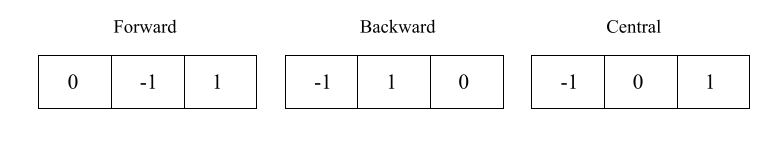
\includegraphics[width=0.75\linewidth]{images/finite_differences.png}
    \caption{Three types of finite differences and their corresponding derivative masks.}
    \label{fig:finite_differences}
\end{figure}

\begin{equation}
    \label{finite_top}
    F_{x}[x_{m},0] =  | I(x_{m},1)-I(x_{m},0) | 
\end{equation}
\begin{equation}
    \label{finite_left}
    F_{y}[0,y_{n}] =  | I(1,y_{n})-I(0,y_{n}) 
\end{equation}
\begin{equation}
    \label{finite_bottom}
    F_{x}[x_{m},h] =  | I(x_{m},h)-I(x_{m},h-1) 
\end{equation}
\begin{equation}
    \label{finite_right}
    F_{y}[w,y_{n}] =  | I(w,y_{n})-I(w-1,y_{n}) 
\end{equation}

With the convoluted pixel values, or, the changes in pixel intensity encoded into both $F_y$ and $F_x$ images, combining them into a single feature map of gradients (vectors with an angle $\theta$) $G$ is as simple as applying the Pythagorean theorem \cite{shidlovskiy_2020_reducing}, as illustrated in figure \ref{fig:pythagorean}, where $ \text{magnitude} = | G(x_{m},y_{n}) | = \sqrt{ F_{y}(x_{m},y_{n})^2+F_{y}(x_{m},y_{n})^2 }$ and $\theta = \arctan \left( \frac{F_{y}(x_{m},y_{n})}{F_{x}(x_{m},y_{n})} \right) $

\begin{figure}
    \centering
    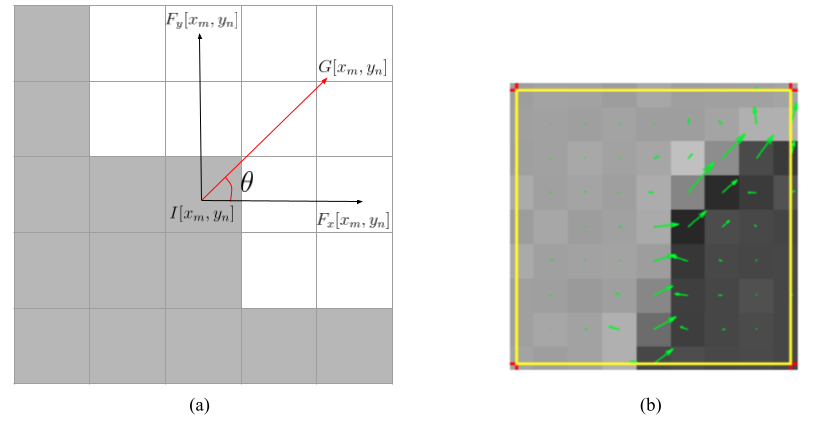
\includegraphics[width=0.75\linewidth]{images/pythagorean.png}
    \caption{(a) Calculation of gradient vector.\\ (b) Visualization of gradient vectors at an edge. Source: \cite{shidlovskiy_2020_reducing}}
    \label{fig:pythagorean}
\end{figure}

\subsubsection{Orientation Binning}

Orientation Binning hopes to achieve an encoding that is both sensitive to variations in local image content while remaining resistant to miniature changes in pose or appearance \cite{dalal_2005_histograms} \cite{shidlovskiy_2020_reducing}. Orientation binning pools gradient orientation information "locally", in a similar way that the SIFT feature detector does \cite{lowe_2004_distinctive}, by first dividing $G$ into a grid of local spatial regions that the authors of the HOG algorithm called cells, as illustrated in figure \ref{fig:cells}.

\begin{figure}
    \centering
    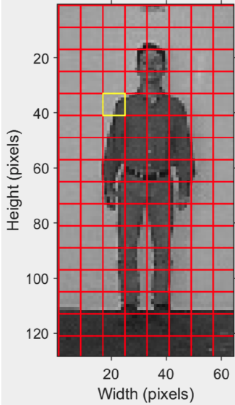
\includegraphics[width=0.2\linewidth]{images/cells.png}
    \caption{A $128\times64$ image divided into a grid of $8\times8$ pixel sized cells. Source: \cite{shidlovskiy_2020_reducing}}
    \label{fig:cells}
\end{figure}

The magnitude of each gradient in $G$ is quantized into a discrete set of $ \omega $ orientation bins, where each bin, $j$, represents a set of angles evenly spaced across the 0°-180° range of possible edge orientations \cite{dalal_2005_histograms}, as done in equation \ref{eq:bin} and shown in figure \ref{fig:histogram_bins}. 

\begin{equation}
    \label{eq:bin}
    j = \left\lfloor  \left( \frac{\theta \omega}{180 \degree} \right) - \frac{1}{2}  \right\rfloor 
\end{equation}

\begin{figure}
    \centering
    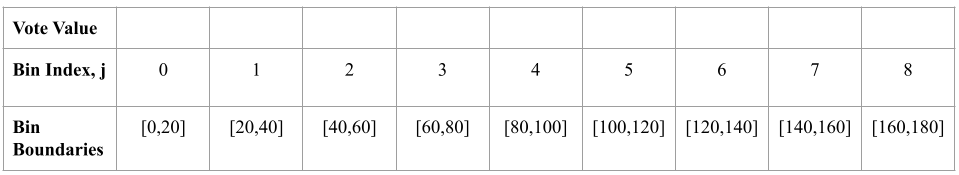
\includegraphics[width=0.75\linewidth]{images/histogram_bins.png}
    \caption{A histogram with 9 equally distributed bins.}
    \label{fig:histogram_bins}
\end{figure}

While a range of 0°-360° may seem to provide more insight into the orientation of an edge, it is generally unnecessary to distinguish between opposite edge directions since object classification is mainly based on detecting boundaries between regions of different intensities. Both edge directions of 90° and 270° convey the same boundary information, just with reversed intensity transitions \cite{shidlovskiy_2020_reducing}. Dalal and Triggs show that using the full 0°-360° range of edge directions not only fails to add useful information but actually decreases a pedestrian classifier's performance \cite{dalal_2005_histograms}, presumably because the wide range of clothing and background color transitions obscure underlying shapes.

\subsubsection{Block Normalisation}

Local contrast normalization in HOG stabilizes gradient representations across varying illumination conditions, enabling the classifier to focus on object structure rather than brightness variations. As shown in figure \ref{fig:normalisation}, the process involves grouping cell histograms into block descriptors $\vec{f{b}} = \{ b{i} \ |\ i=1,2,\dots, c_w \cdot c_h \}$, where $c_w$ and $c_h$ are block dimensions. While multiple normalization schemes exist ($\mathrm{L1}$, $\mathrm{L1-sqrt}$, $\mathrm{L2}$, $\mathrm{L2-hys}$), their performance differences in pedestrian detection are minimal, with $\mathrm{L2-hys}$ showing slight advantages \cite{dalal_2005_histograms}.

\begin{figure}
    \centering
    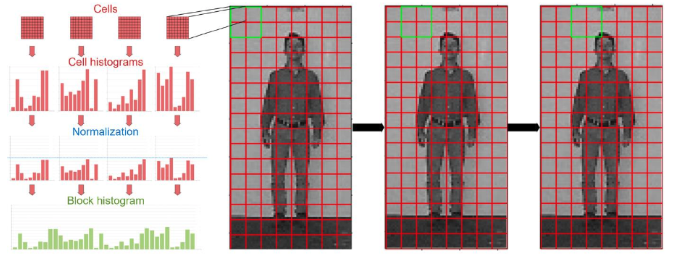
\includegraphics[width=0.75\linewidth]{images/normalisation.png}
    \caption{Construction of block descriptors with (2,2) cells per block. Source: \cite{shidlovskiy_2020_reducing}}
    \label{fig:normalisation}
\end{figure}

Blocks in HOG typically overlap, with overlap percentages determined by the block stride: $(1-\frac{\text{horizontal block stride}}{\text{block width}})\%$ horizontally and $(1-\frac{\text{vertical block stride}}{\text{block height}})\%$ vertically. Though this results in multiple normalizations of the same cell histograms, the redundant block descriptor vectors $\vec{f_b}$ significantly enhance detection performance \cite{dalal_2005_histograms}.

\subsubsection{Feature Vector Dimensionality}\label{sec:feature_vector_dimensionality}

In real world applications, pedestrians can appear at different scales, positions, and orientations within an image, necessitating a systematic search across the entire image space. A sliding detection window of dimensions $W_h$ and $W_w$ does exactly that, scanning the image in a grid-like fashion, shifting over both horizontal and vertical axes. As the window moves across the image, the feature descriptors $\vec{f_b}$ within each bounded block's region are computed, normalized, and combined into a larger feature vector, $\vec{L}$, which represents the entire window and is used as input to a classifier, as illustrated in figure \ref{fig:hog_pipeline}. 

\begin{figure}
    \centering
    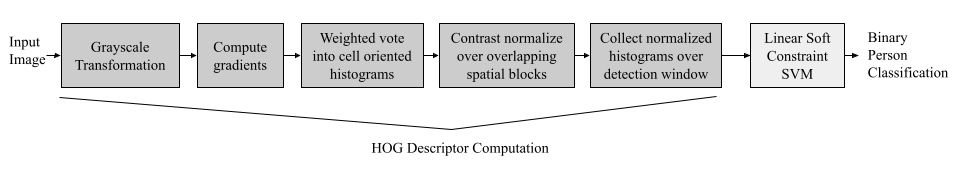
\includegraphics[width=1\linewidth]{images/HOG Pipeline.png}
    \caption{An overview of the HOG feature extraction chain. Source: Adapted by me from \cite{dalal_2005_histograms}}
    \label{fig:hog_pipeline}
\end{figure}

The feature vector $\vec{L}$ has dimensionality $d$, representing the total number of gradient features extracted from the image region. This vector exists in a $d$-dimensional feature space ($\vec{L} \in \mathcal{R}^{d}$), where higher dimensionality generally provides more discriminative power for distinguishing pedestrians—though this relationship is not always beneficial, as discussed in section \ref{sec:curse_of_dimensionality}.

\begin{figure}
    \centering
    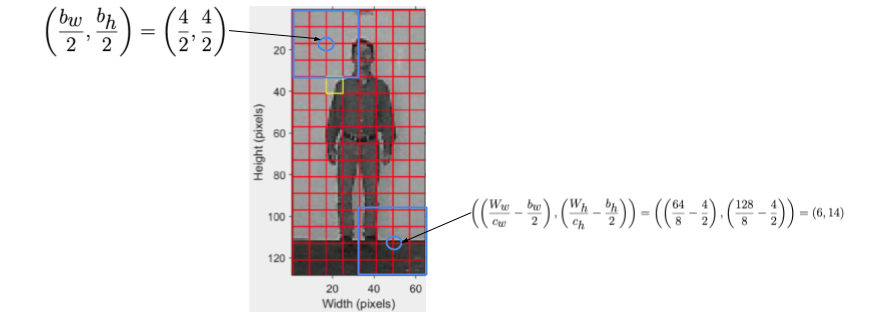
\includegraphics[width=1\linewidth]{images/Center Coordinates.png}
    \caption{A $128\times64$ image with (8,8) cells and (4,4) cells. If $b_w,b_h,c_w,c_h,W_w,W_w\in2\mathbb{Z}$, it is simple to calculate the center coordinates of each block. Source: Adapted by me from \cite{shidlovskiy_2020_reducing}}
    \label{fig:center_coords}
\end{figure}

The dimensionality $d$ of feature vector $\vec{L}$ is determined by:
\begin{enumerate}
    \item Block descriptor size: ($c_w \cdot c_h \cdot \omega$), where $c_w \cdot c_h$ is the number of cells per block and $\omega$ is orientation bins per cell
    \item Total block count: calculated from horizontal and vertical stride values ($s_w$, $s_h$) within the detection window
\end{enumerate}

$b_w,b_h,c_w,c_h,W_w,W_w\in2\mathbb{Z}$ must hold to ensure complete window coverage, as shown in figure \ref{fig:center_coords}. These relationships are formalized in equation \ref{vector_dimensions}.

\begin{equation}
    \label{vector_dimensions}
    \begin{split}
    d &= \left\lfloor \frac{\frac{W_w}{c_w}-2\cdot\frac{b_w}{2}+1}{s_w} \right\rfloor\left\lfloor \frac{\frac{W_h}{c_h}-2\cdot\frac{b_h}{2}+1}{s_h} \right\rfloor\cdot b_w b_h\omega \\ &= \left\lfloor  \frac{W_w- c_w(b_w-1)}{s_w c_w}  \right\rfloor \left\lfloor   \frac{W_h -c_h(b_h -1)}{s_h c_h} \right\rfloor b_w b_h\omega
    \end{split}
\end{equation}

\subsection{The Curse of Dimensionality}\label{sec:curse_of_dimensionality}

While it would be reasonable to intuitively to assume that the more information, or vector dimensions, a machine is provided during training, the more accurate it would be at classification tasks, the classic "curse of dimensionality" problem shows that this is not necessarily the case \cite{jain_1982_39} \cite{friedman_1997_on}, as overfitting, the process of fitting to noise rather than underlying patterns, \cite{overfitting} occurs when the amount of "specific information" (the dimensions of each data point's vector $\vec{L}$) is significantly greater than "global information" (the amount of data points in a data set) \cite{overfitting} \cite{liu_2016_overfitting}, as shown in figure \ref{fig:curse_dim}. 

\begin{figure}
    \centering
    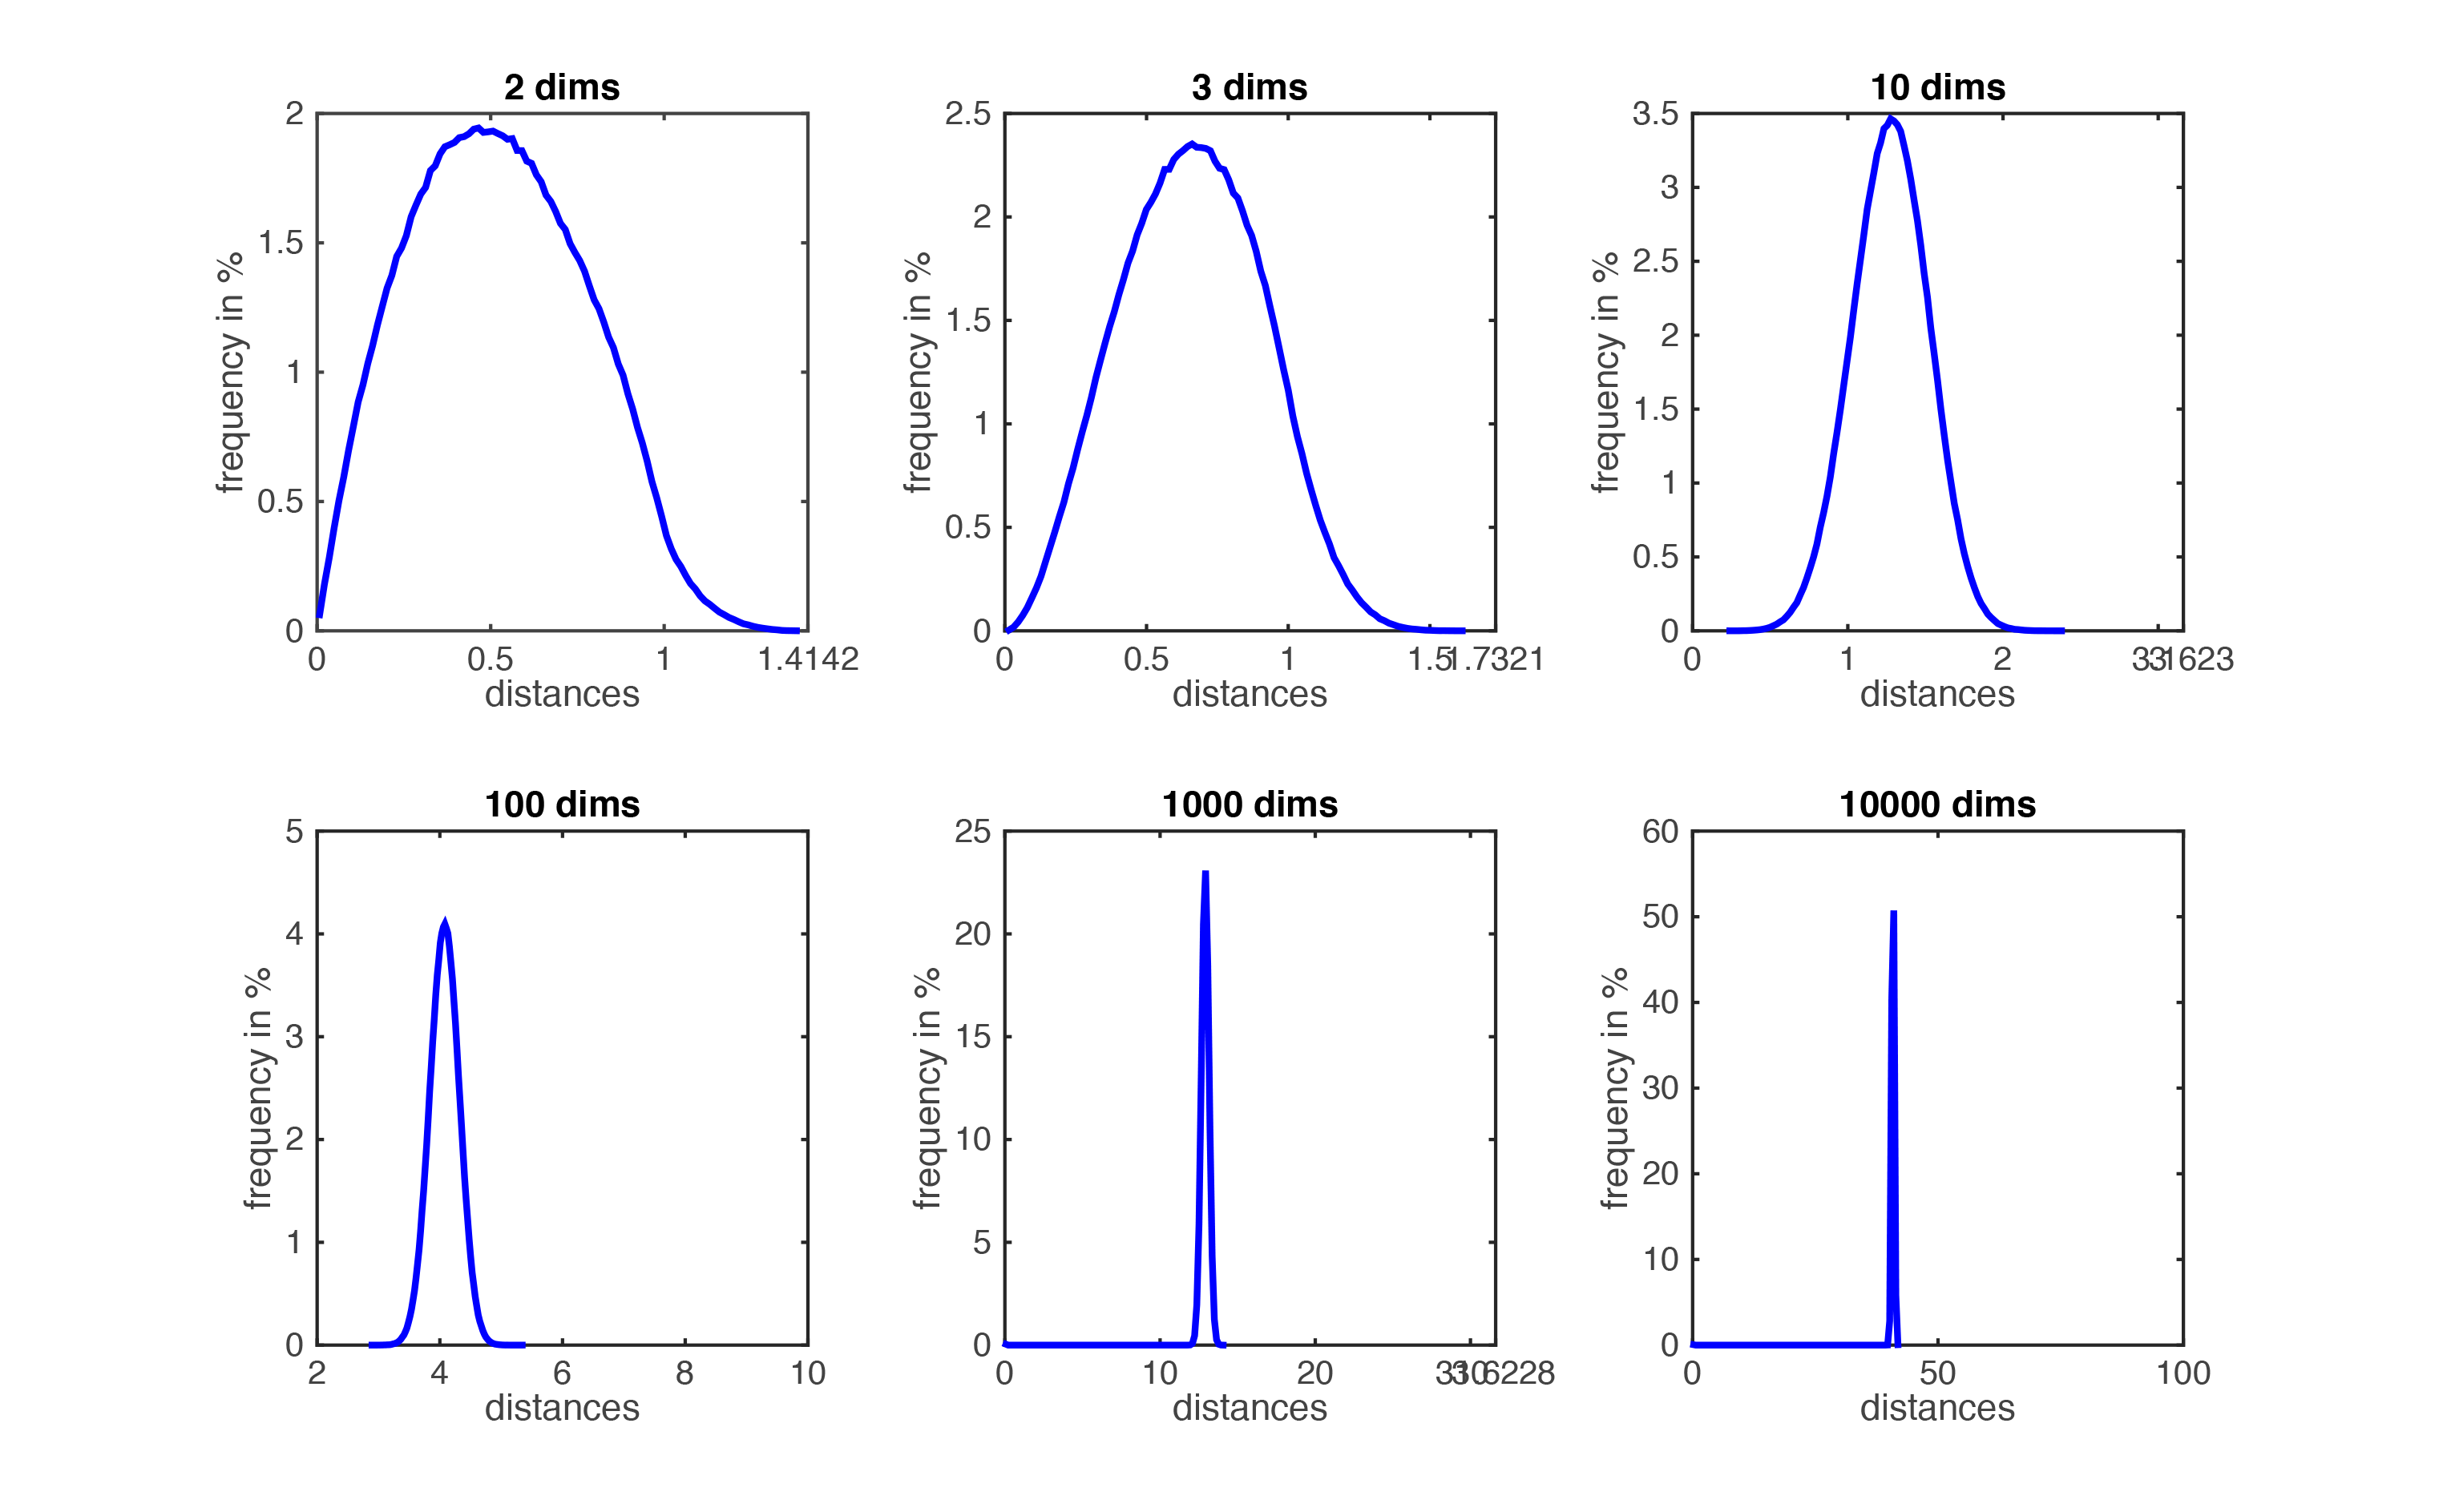
\includegraphics[width=\linewidth]{images/cursefigure.png}
    \caption{The histogram plots show the distributions of all pairwise distances between randomly distributed points within $d$-dimensional unit squares. As the number of dimensions $d$ grows, all distances concentrate within a very small range. Source: \cite{cornell_curse_notes}
}
    \label{fig:curse_dim}
\end{figure}

\subsection{Supervised Machine Learning}\label{sec:supervised_ml}

Machine Learning (ML), on a surface level, is the study of algorithms that are designed to produce outputs without an explicit instruction set generated by a person but rather with reference to the patterns or correlations found in data \cite{what_is_ml}. 

In that respect, supervised ML, a subset of ML, attempts to make predictions from previously observed labeled data, which provides the correct output that an algorithm should produce for each data point \cite{supervised_learning}. Classifiers are a common application of supervised ML, where the goal is to predict the class of a new data point based on the classes of previously observed data points \cite{derek_2020_svm}. For example, does a window in an image contain a pedestrian or not?

Classifier training data is formally defined as $D={ (x_{1},y_{1}),\dots,(x_{n},y_{n}) }$, where each feature vector $x_i$ belongs to a $d$-dimensional space ($x_i\in \mathcal{R}^d$) and each label $y_i$ belongs to a label space $\mathcal{C}$ \cite{supervised_learning}. For the purpose of binary classification, such as pedestrian detection, the label space contains just two values: $+1$ for pedestrians and $-1$ for non-pedestrians \cite{cornell_svm}. Since each feature vector $x_i$ corresponds to a HOG descriptor $\vec{L}$, any change in the HOG parameters discussed in section \ref{sec:feature_vector_dimensionality} alters the dimensionality of $\vec{L}$ and consequently requires training a new classifier model with appropriately dimensioned feature vectors.

\subsection{Support Vector Machines}

Support Vector Machines (SVM) are widely adopted supervised ML algorithms, particularly well-suited for classifying points in high-dimensional feature spaces \cite{ng_support} (like those generated by HOG descriptors), a property which has been demonstrated across various domains including brain disorder diagnosis \cite{derek_2020_svm}, neuroimaging analysis \cite{svm_mri}, and, notably, pedestrian detection \cite{dalal_2005_histograms}.

An SVM finds the optimal boundary, called a hyperplane ($\mathcal{H}={ x|w^\top x + b = 0 }$), to separate data classes by maximizing the margin between the boundary and the nearest data points (support vectors) \cite{derek_2020_svm} \cite{cornell_svm_notes}. Unlike similar algorithms like the Perceptron \cite{cornell_perceptron}, SVMs uniquely prioritize margin maximization \cite{ng_support}. Figure \ref{fig:hyperplane} illustrates in 2D, where the hyperplane becomes a line, $w$ represents the vector perpendicular to this line, and $b$ determines the line's intercept with the y-axis.

% TODO: Seperate
\begin{figure}
    \centering
    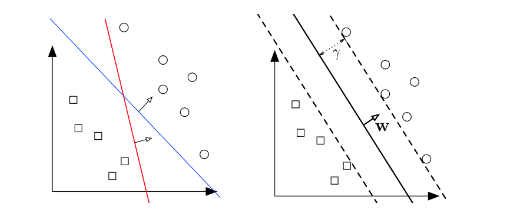
\includegraphics[width=0.75\linewidth]{images/hyperplane.png}
    \caption{Two 2D spaces where data points have 2 features. (Left:) The multiple possibles hyperplanes of an algorithm like the perceptron. (Right:) The only possible margin maximizing hyperplane of the SVM algorithm. Source: \cite{cornell_svm_notes}}
    \label{fig:hyperplane}
\end{figure}

The maximum margin hyperplane optimizes classifier generalization (ability to correctly classify unseen data) by maximizing the distance $\gamma$ between support vectors and the decision boundary, which is defined using the hyperplane's weight and bias parameters in equation \ref{margin_expr} \cite{cornell_svm}.

\begin{equation}\label{margin_expr}
    \gamma(w,b)=\min_{x\in D} \frac{|w^\top x + b|}{||w||_{2}}
\end{equation}

\begin{figure}
    \centering
    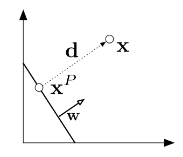
\includegraphics[width=0.35\linewidth]{images/hyperplane_geometry.png}
    \caption{The projection of a data point onto the hyperplane. Source: \cite{cornell_svm_notes}}
    \label{fig:hyperplane_geometry}
\end{figure}

With a defined margin, finding the optimal hyperplane can be formulated as a concrete optimization problem: maximize $\gamma$ while ensuring all data points lie on the "correct" side of the hyperplane. For any data point $x_i$,  $w^\top x_i + b$ determines the point's signed distance relative to the hyperplane $\mathcal{H}$. As all $x_i$ above $\mathcal{H}$ are coupled with $y_i=+1$ and those below with $y_i=-1$, the expression $y_{i}(w^\top x_{i}+b)$ should be positive for all correctly classified points \cite{ng_support}, providing a mathematical foundation for the optimization constraint in \ref{hyper_inequality}.

\begin{equation}\label{hyper_inequality}
y_{i}(w^\top x_{i}+b)\ge 0 \quad 
\end{equation}
%TODO: Should I expand more on the concrete form of how this optimization problem looks?

\subsubsection{Soft SVM Constraints}\label{sec:soft_constraint_svm}

While the maximum margin hyperplane can be found by minimizing $||w||_{2}$ with hard constraints using QCQP or SMO algorithms \cite{chang_lin_2011_libsvm}, pedestrian datasets contain noise \cite{Zhang_2016_CVPR} and humanoid objects with pedestrian-like features \cite{karthika_2020_addressing}, as shown in figures \ref{fig:pedestrian_features}, \ref{fig:manequin_features}. Given these real-world complications and overlapping class features (figure \ref{fig:outliers}), soft-margin SVM allowing controlled misclassification provides more realistic classification accuracy \cite{dalal_2005_histograms} \cite{cornell_svm_continued}

\begin{figure}
    \centering
    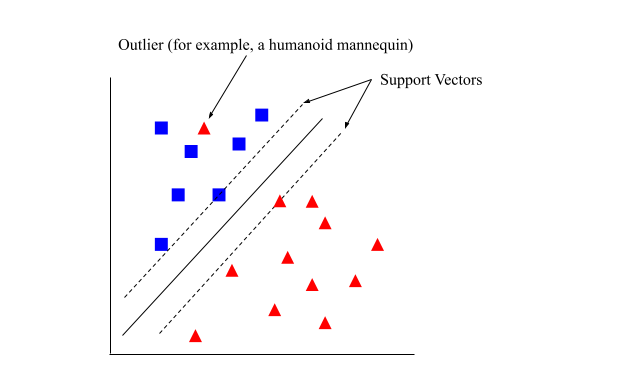
\includegraphics[width=0.75\linewidth]{images/outliers.png}
    \caption{A Data set with two classes and an outlier.}
    \label{fig:outliers}
\end{figure}


\begin{figure}
    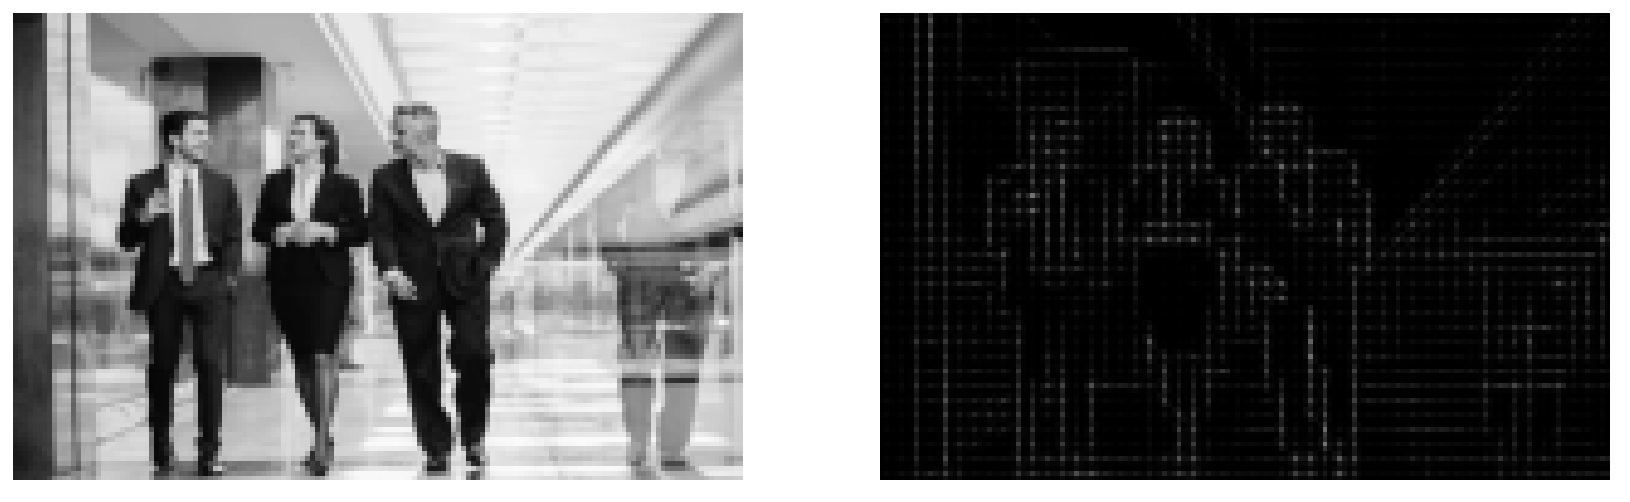
\includegraphics[width=0.75\linewidth]{features-1.png}
    \caption{(Left:) Three people/pedestrians in a building. Source: \cite{person_img} (Right:) The computed HOG features of the image}
    \label{fig:pedestrian_features}
\end{figure}

\begin{figure}
    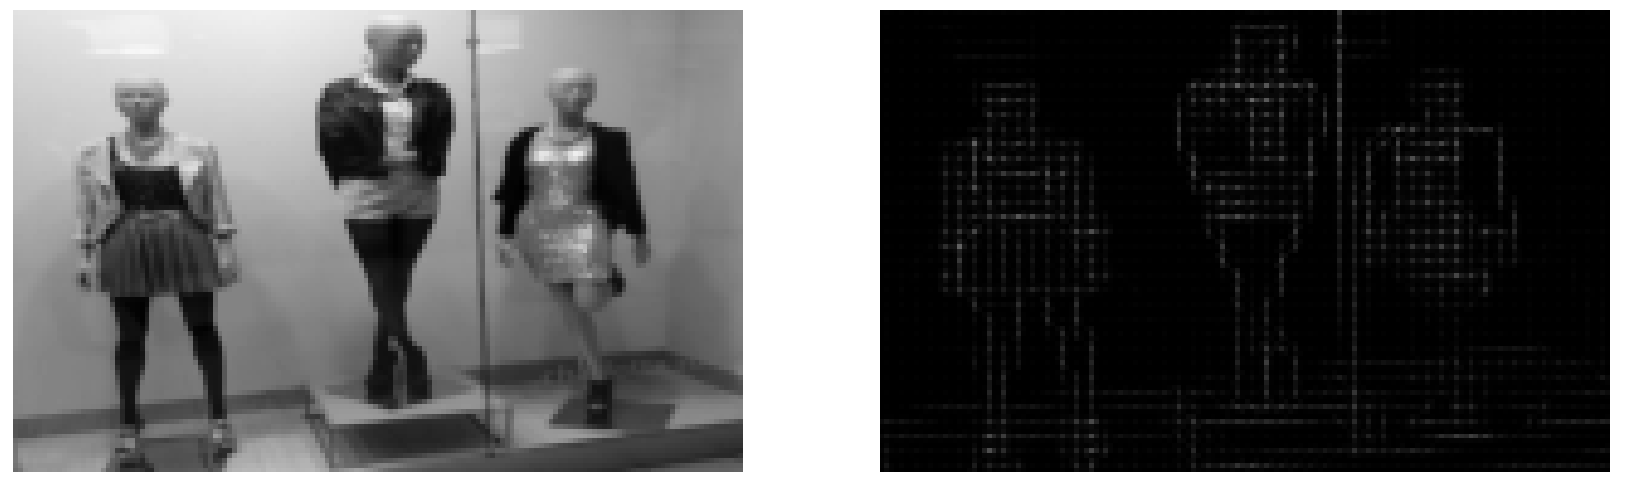
\includegraphics[width=0.75\linewidth]{features-2.png}
    \caption{(Left:) Three mannequins in a store window. Source: \cite{mannequin_img} (Right:) The computed HOG features of the image}
    \label{fig:manequin_features}
\end{figure}

\subsection{Model Evaluation Metrics}

\subsubsection{The Basic Confusion Matrix Rates}
In essence, all evaluation metrics of binary classification rely on the values of the confusion matrix, a $2 \times 2$ contingency table where the positive elements correctly classified as positives are called true positives (TP), the negative elements wrongly classified as positive - false positives (FP), the negative elements correctly classified as negatives - true negatives (TN), and the positive elements wrongly classified as negatives - false negatives (FN), as shown in figure \ref{fig:conf_matrix}. \cite{chicco_eval_2023}. 

\begin{figure}
    \centering
    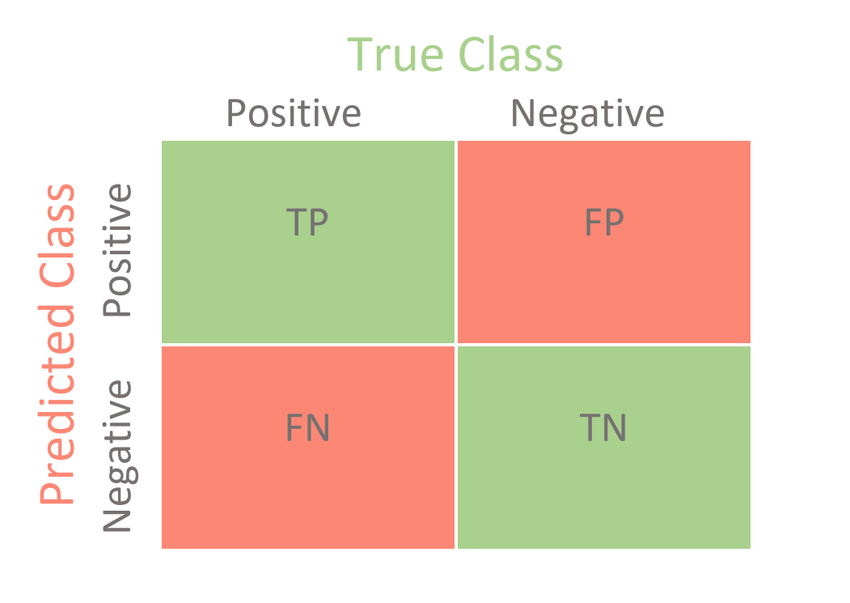
\includegraphics[width=0.5\linewidth]{images/conf_matrix.png}
    \caption{An example of a confusion matrix for binary classification. Source: \cite{conf_matrix}}
    \label{fig:conf_matrix}
\end{figure}

The four basic rates for confusion matrices are as follows \cite{chicco_eval_2023}:
\begin{enumerate}
    \item Sensitivity, or True Positive Rate, $\mathrm{TPR}=\frac{\mathrm{TP}}{\mathrm{TP}+\mathrm{FN}}$

    \item Specificity, or True Negative Rate, $\mathrm{TNR}=\frac{\mathrm{TN}}{\mathrm{TN}+\mathrm{FP}}$
    
    \item Precision, or Positive Predictive Value, $\mathrm{PPV}=\frac{\mathrm{TP}}{\mathrm{TP}+\mathrm{FP}}$
    
    \item Negative Predictive Value, $\mathrm{PPV}=\frac{\mathrm{TN}}{\mathrm{TN}+\mathrm{FN}}$
\end{enumerate} 

\subsubsection{Confidence Threshold Curves}

Scoring classifiers (like logistic regression \cite{cornell_log_regression_notes}) output real-valued predictions that generate confusion matrices based on a threshold $\tau$ \cite{chicco_jurman_2020_mcc_f1}, visualized through valuable ROC or DET curves \cite{martin1997det}, with DET being preferred for pedestrian detection \cite{dalal_2005_histograms} \cite{dollar_2012_pedestrian}. While SVMs do not produce probabilistic outputs, distances to the hyperplane may serve as proxy confidence measures, as cross-validation in Platt Scaling \cite{platt1999probabilistic} for true probability estimation is computationally expensive and potentially inconsistent with SVM predictions \cite{scikit-learn_svm}.

\subsubsection{Matthew's Correlation Coefficient}

Despite their prevalence in pedestrian detection \cite{dalal_2005_histograms} \cite{dollar_2012_pedestrian} \cite{dollar_2009_pedestrian}, ROC/DET curves ignore precision \cite{chicco_eval_2023} \cite{chicco_jurman_2020_mcc_f1}. While precision-recall curves address this limitation \cite{chicco_jurman_2020_mcc_f1}, Matthew's Correlation Coefficient (MCC, as defined in appendix \ref{appendix:matthews_correlation}) provides a superior single metric by incorporating all confusion matrix elements and offering higher discriminative power for binary classifier evaluation \cite{Maier_Hein_2024_mcc_proposal} \cite{chicco_eval_2023}, making it, alongside a corresponding MCC-F1 curve from figure \ref{fig:mcc_f1_example}, the primary metrics for this investigation.
% TODO
\begin{figure}
    \centering
    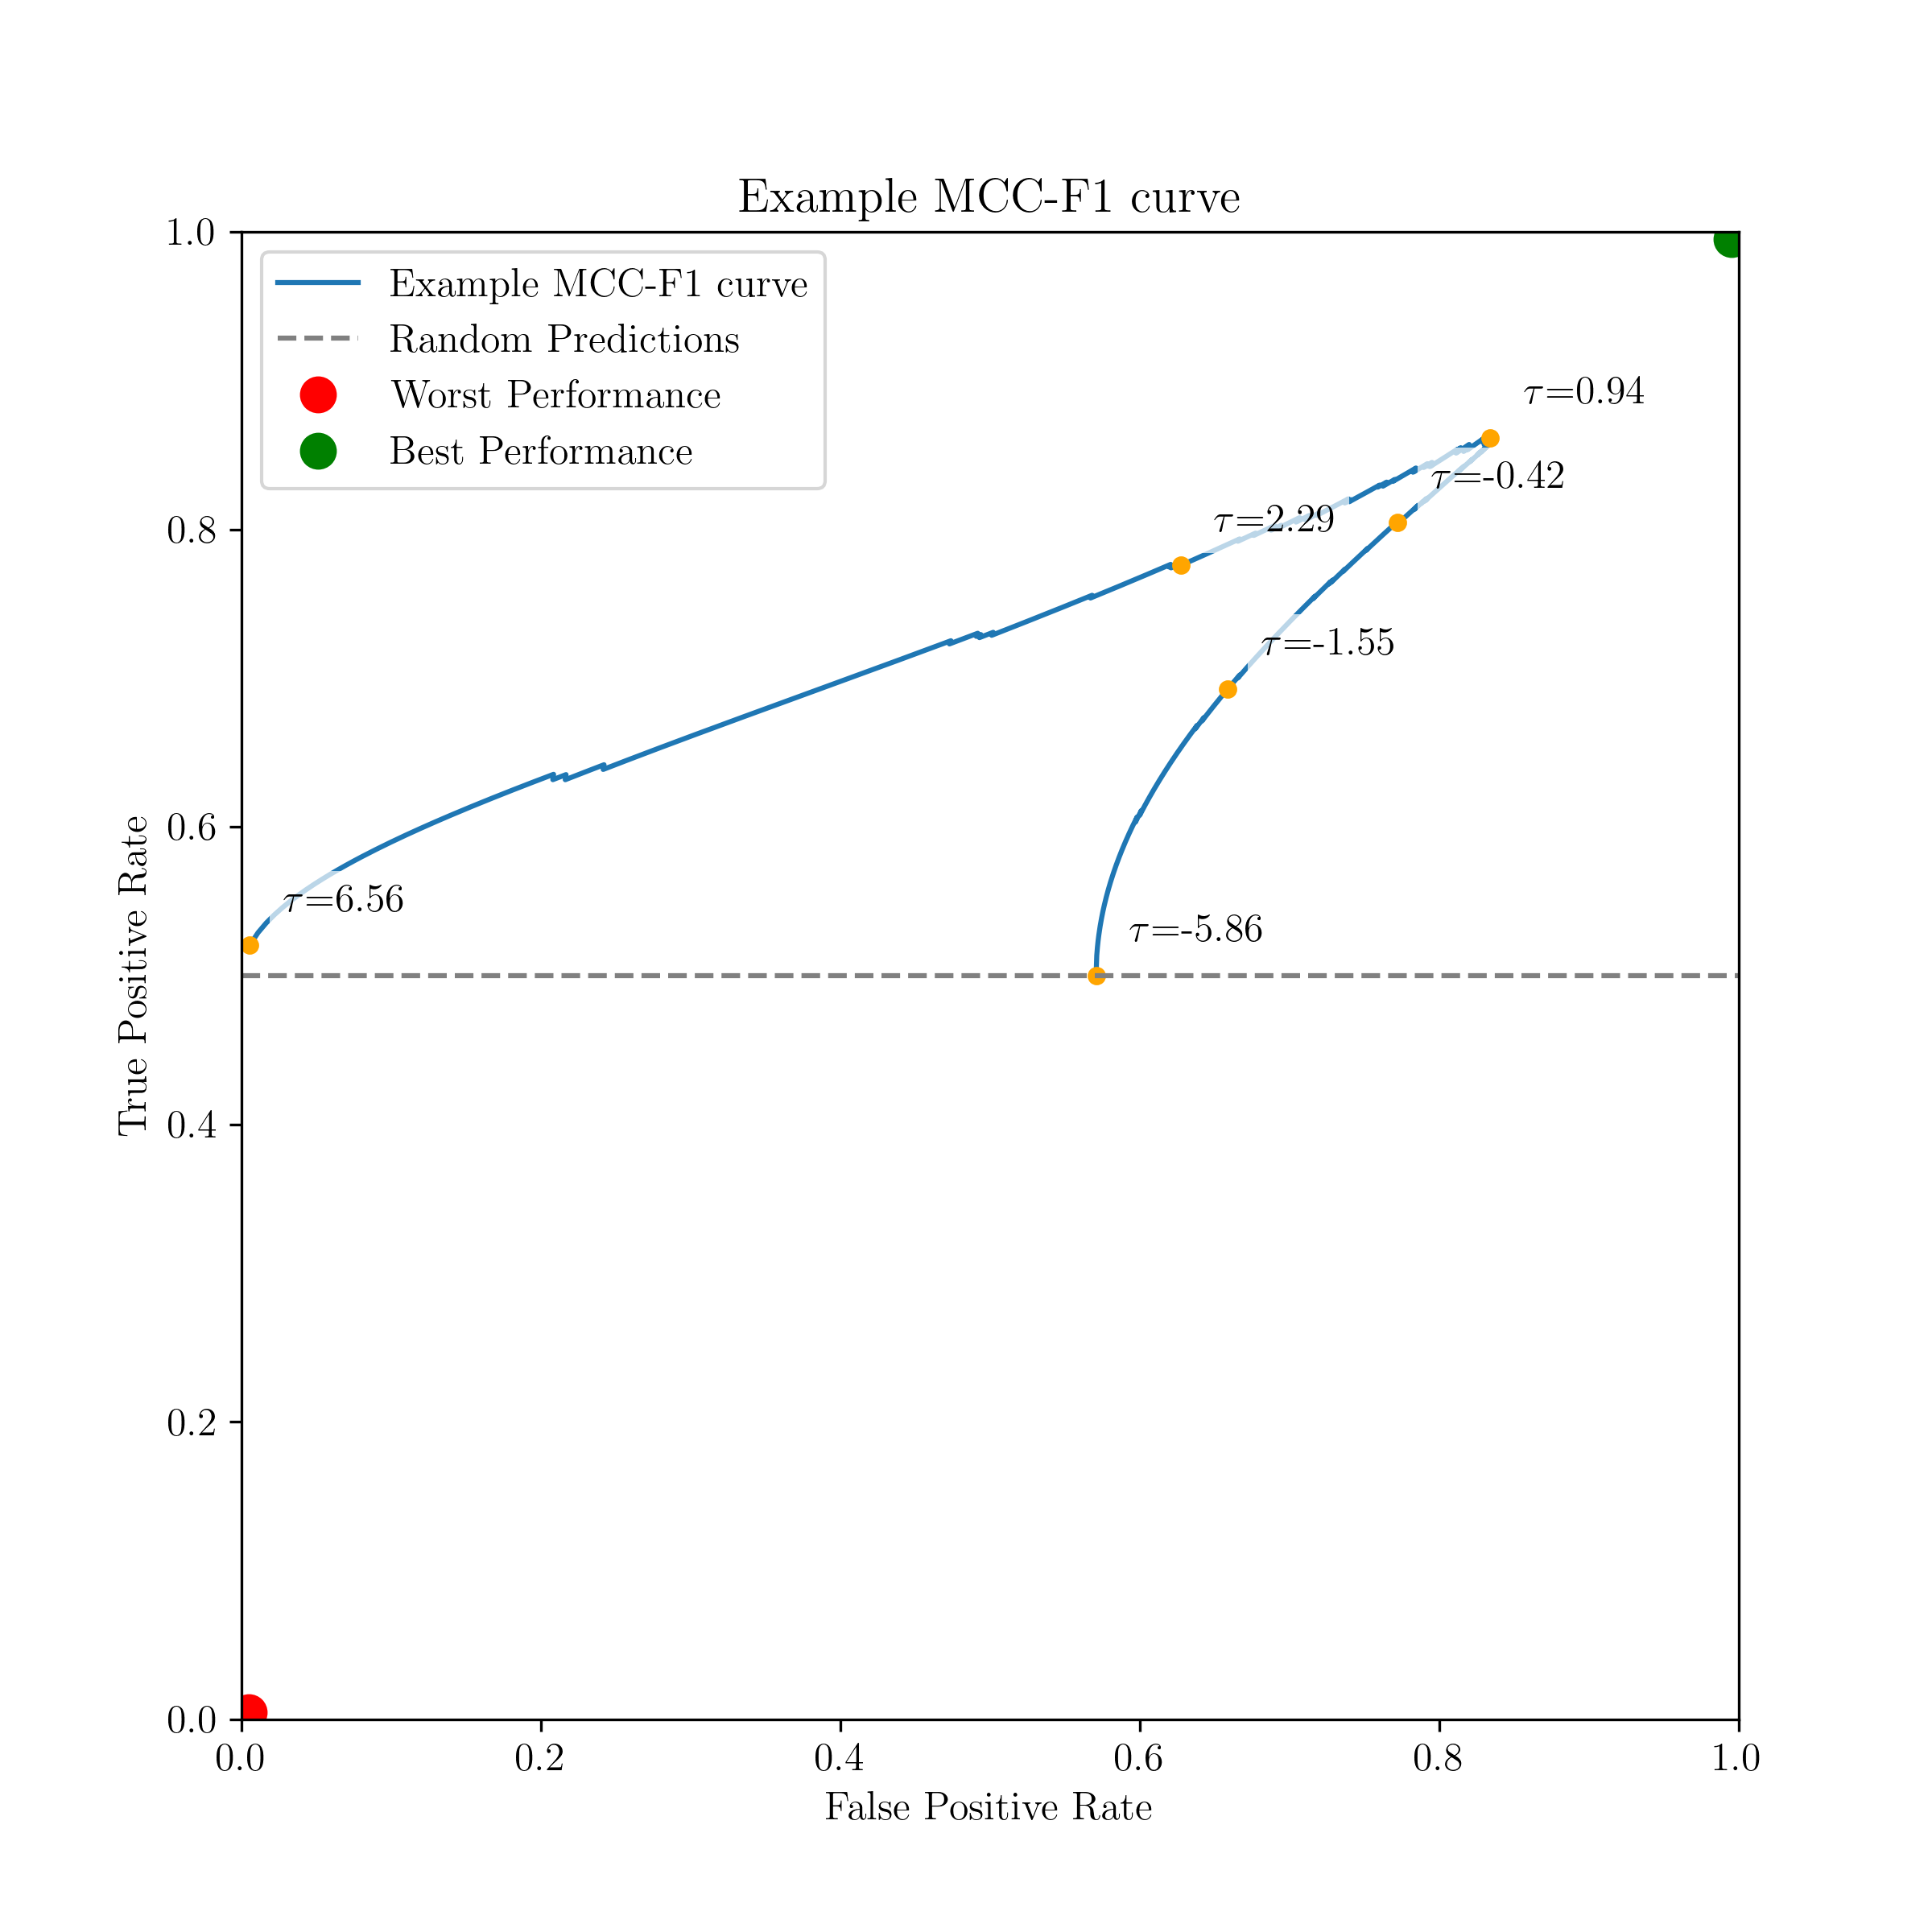
\includegraphics[width=0.75\linewidth]{images/mcc_f1_example.png}
    \caption{Unit-normalized MCC plotted against the F1 score (the harmonic mean between precision and recall). 6 various threshold $\tau$ values are scattered along the curve. Source: Code in appendix \ref{appendix:mcc_f1_curves}}
    \label{fig:mcc_f1_example}
\end{figure}

Nevertheless, since much of the literature on pedestrian detection and classification has historically relied on metrics like AUC-ROC, Average Precision and simple Accuracy \cite{dalal_2005_histograms} \cite{dollar_2012_pedestrian}, they are retained to facilitate direct and simple comparison with previous studies.

\subsubsection{McNemar's Test for Pairwise Classifier Comparison}

While $5 \times 2$ Cross Validation was traditionally preferred for pairwise classifier comparison \cite{dietterich_1998_mcnemar}, McNemar's test offers a more efficient and scalable with large datasets alternative, requiring only one execution rather than ten \cite{raschka_2018_mcnemar}. McNemar's test evaluates statistical significance in classifier performance by analyzing their disagreement patterns from a confusion matrix, like the one in figure \ref{fig:confusion_mcnemar}, and computing a p-value, the probability that the observed difference in performance is due to chance, based on chi-square statistics \cite{dietterich_1998_mcnemar}, with $p \ge 0.05$ typically indicating no significant performance difference \cite{raschka_2018_mcnemar} \cite{dietterich_1998_mcnemar}.

\begin{figure}
    \centering
    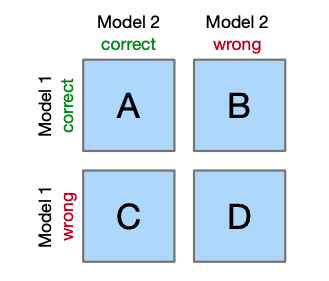
\includegraphics[width=0.5\linewidth]{images/mcnemar_matrix.png}
    \caption{Confusion matrix layout in the context of McNemar's test. Source: \cite{raschka_2018_mcnemar}, code in appendix \ref{appendix:mcnemar}}
    \label{fig:confusion_mcnemar}
\end{figure}


